\documentclass[12pt,a4paper]{article}

\usepackage[T1]{fontenc}
\usepackage{lmodern}
\usepackage{microtype}
\usepackage[a4paper,margin=23mm]{geometry}
\usepackage{amsmath,amssymb}
\usepackage{graphicx}
\usepackage{booktabs,tabularx,array,longtable}
\usepackage[table]{xcolor}
\usepackage{enumitem}
\usepackage{caption}
\usepackage{float}
\usepackage{pdflscape}
\usepackage{xurl}
\usepackage{listings}
\usepackage{tikz}
\usetikzlibrary{positioning,arrows.meta,shapes.geometric}
\usepackage[numbers,sort&compress]{natbib}
\usepackage[colorlinks=true,allcolors=blue!55!black]{hyperref}

\newcommand{\ProjName}{CrashGuard}
\newcommand{\TeamMemberA}{Adheesh Garg}
\newcommand{\TeamRegA}{23BCT0122}
\newcommand{\TeamMemberB}{Aastha Gupta}
\newcommand{\TeamRegB}{23BCT0082}
\newcommand{\TeamMemberC}{Ayan Gatani}
\newcommand{\TeamRegC}{23BCT0059}


% Generated by analysis/evaluate.py. Do not edit by hand.
\newcommand{\SimulationSeed}{20260828}
\newcommand{\SimulationEvents}{675}
\newcommand{\SimulationSamples}{675,000}
\newcommand{\PositiveEvents}{150}
\newcommand{\NegativeEvents}{525}
\newcommand{\VTwoSensitivity}{76.0\%}
\newcommand{\VTwoSpecificity}{100.0\%}
\newcommand{\VTwoFOne}{0.864}
\newcommand{\VTwoTP}{114}
\newcommand{\VTwoTN}{525}
\newcommand{\VTwoFP}{0}
\newcommand{\VTwoFN}{36}
\newcommand{\VTwoSensitivityLow}{68.6\%}
\newcommand{\VTwoSensitivityHigh}{82.1\%}
\newcommand{\VTwoSpecificityLow}{99.3\%}
\newcommand{\VTwoConfirmationDelayMs}{2310}
\newcommand{\VTwoImpactThreshold}{2.00}
\newcommand{\VTwoLowImpactThreshold}{0.35}
\newcommand{\VTwoRotationThreshold}{90}
\newcommand{\VTwoTiltThreshold}{55}
\newcommand{\VTwoRestHoldMs}{2000}
\newcommand{\VTwoCorrelationMs}{750}
\newcommand{\VTwoRideQualificationMs}{1000}
\newcommand{\VTwoRideMemoryMs}{5000}
\newcommand{\BaselineSensitivity}{89.3\%}
\newcommand{\BaselineSpecificity}{45.0\%}
\newcommand{\BaselineFOne}{0.468}
\newcommand{\LegacySensitivity}{26.0\%}
\newcommand{\LegacySpecificity}{100.0\%}
\newcommand{\LegacyFOne}{0.413}
\newcommand{\LegacyConfirmationDelayMs}{3120}
\newcommand{\ExternalFallCount}{4}
\newcommand{\ExternalManoeuvreCount}{7}
\newcommand{\ExternalFourGPass}{0}
\newcommand{\ExternalTwoHundredPass}{0}
\newcommand{\ExternalVTwoImpactPass}{4}
\newcommand{\ExternalVTwoRotationPass}{4}


\newcommand{\degree}{\ensuremath{^{\circ}}}
\newcommand{\pass}{\cellcolor{green!14}\textbf{Pass}}
\newcommand{\partialpass}{\cellcolor{orange!18}\textbf{Partial}}
\newcommand{\notmeasured}{\cellcolor{gray!15}\textbf{Not measured}}
\renewcommand{\arraystretch}{1.15}
\setlist{nosep,leftmargin=*}
\captionsetup{font=small,labelfont=bf}
\setlength{\bibsep}{2pt}
\bibliographystyle{IEEEtran}
\lstset{basicstyle=\ttfamily\footnotesize,frame=single,breaklines=true,
  columns=fullflexible,backgroundcolor=\color{gray!5},rulecolor=\color{gray!35}}

\title{\textbf{\ProjName: IoT Integration, Testing, and Performance Evaluation}\\
\large Crash Detection and Rider-Cancellable Emergency Alert System}
\author{\TeamMemberA{} (\TeamRegA) \and
        \TeamMemberB{} (\TeamRegB) \and
        \TeamMemberC{} (\TeamRegC)}
\date{Programming for IoT Boards Lab (BCSE312P)\\
Class VL2026270103137 \quad Faculty: Syamasudha Veeragandham (22727)\\
Assessment 6, Review 3 \quad 4 September 2026}

\begin{document}
\maketitle

\begin{abstract}
This report evaluates CrashGuard, an ESP32 and MPU-6050 prototype that detects
fall-like motorcycle motion, activates a local LED and piezo alarm, gives the
rider 15 seconds to cancel, and then attempts a Blynk IoT event. Because
physical hardware is unavailable, the evidence combines exact-code native
replay, 675 deterministic six-axis events, four public powered-two-wheeler
falls, seven public critical manoeuvres, target compilation, and a fresh
three-scenario Wokwi virtual-hardware run. Ten normal, boundary, abnormal, and
fault-oriented cases are reported. CrashGuard obtains 94.7\% simulated event
accuracy, 76.0\% sensitivity, 100.0\% observed specificity, and a 2.31 s median
confirmation delay. An acceleration-only comparison is more sensitive
(89.3\%) but raises false alarms on 55.0\% of simulated non-crash events.
The report also defines the Blynk event, dashboard mapping, communication
chain, fault responses, deviations, and future validation plan. No physical
crash accuracy, phone-notification receipt, network latency, or measured
battery life is claimed.
\end{abstract}

\clearpage
\tableofcontents
\clearpage

\section{Assessment objective and coverage}

Assessment 6 requires integration, testing, performance evaluation, IoT
communication, a dashboard, fault handling, expected-versus-actual analysis,
and future enhancements. Table~\ref{tab:coverage} maps each requirement to the
evidence in this report.

\begin{table}[H]
\centering
\small
\caption{Assessment requirement coverage.}
\label{tab:coverage}
\begin{tabularx}{\textwidth}{@{}p{0.27\textwidth}X p{0.16\textwidth}@{}}
\toprule
Requirement & Evidence & Section \\
\midrule
At least five tests & Ten normal, boundary, abnormal, and fault-oriented cases & \ref{sec:testplan}--\ref{sec:testresults} \\
Expected versus actual & Acceptance criteria, actual output, status, and deviation table & \ref{sec:testresults}, \ref{sec:deviations} \\
Performance comparison & Accuracy, sensitivity, false-positive rate, F1, delay, and resources & \ref{sec:performance} \\
IoT communication & Sensor-to-controller-to-network-to-Blynk-to-user chain & \ref{sec:iot} \\
Dashboard / UI & Reproducible replay dashboard and Blynk widget specification & \ref{sec:dashboard} \\
Two fault conditions & Sensor/I\textsuperscript{2}C and Wi-Fi/Blynk failure behavior & \ref{sec:faults} \\
Future enhancements & Prioritized hardware, communication, security, and model work & \ref{sec:future} \\
\bottomrule
\end{tabularx}
\end{table}

The previous review's suggestions are retained: CrashGuard is treated as one
system rather than a sequence of named versions; its thresholds are compared
with public motorcycle data; the supplied human-fall paper is audited rather
than copied; the firmware and replay share decision logic; and Wokwi and cloud
claims are bounded to what was actually tested.

\section{System under test}

\subsection{Purpose and hardware}

CrashGuard is mounted on the motorcycle handlebar. Its MPU-6050 supplies
three-axis acceleration and angular rate at 100 Hz. The ESP32 calculates
acceleration magnitude, angular-rate magnitude, and tilt relative to the
stationary startup gravity vector. GPIO26 drives the warning LED; GPIO25 drives
a physical 5 V passive piezo through a transistor; GPIO27 reads the active-low
cancel button; and GPIO34 monitors the divided battery voltage. The MPU-6050 is
configured for $\pm16g$ and $\pm2000\degree$/s to reduce immediate saturation
under rapid motion~\cite{mpu6050datasheet}. GPIO34 is an ADC1 input and remains
usable while Wi-Fi is active~\cite{esp32datasheet}.

\begin{table}[H]
\centering
\small
\caption{Interfaces of the evaluated prototype.}
\begin{tabularx}{\textwidth}{@{}p{0.19\textwidth}p{0.23\textwidth}X@{}}
\toprule
Subsystem & Interface & Evaluated role \\
\midrule
MPU-6050 & I\textsuperscript{2}C, GPIO21/22 & Six-axis source at 100 Hz \\
Local alarm & GPIO26 LED, GPIO25 piezo & Immediate rider-visible/audible warning \\
Rider input & GPIO27, internal pull-up & Cancels pending cloud alert \\
Battery sense & GPIO34 through 1:2 divider & Startup voltage observation \\
Network & ESP32 Wi-Fi station & Phone hotspot or Wokwi-GUEST \\
Cloud/user & Blynk IoT SSL client & Event timeline and notification attempt \\
\bottomrule
\end{tabularx}
\end{table}

\subsection{CrashGuard decision sequence}

The detector does not equate a single shock with a crash. It first requires
one second of ride-like activity and remembers it for five seconds. A candidate
then begins when acceleration magnitude $A$ satisfies $A\geq2.0g$ or
$A\leq0.35g$. Angular motion $\Omega\geq90\degree$/s must occur within a
750 ms correlation interval, in either order. Finally, tilt must reach
$55\degree$ while $0.70g\leq A\leq1.30g$ and
$\Omega\leq30\degree$/s continuously for two seconds. A candidate that does
not establish final rest within six seconds is rejected.

\begin{figure}[H]
\centering
\begin{tikzpicture}[
  node distance=7mm and 7mm,
  state/.style={draw,rounded corners,align=center,minimum width=25mm,
    minimum height=10mm,fill=blue!5,font=\small},
  arrow/.style={-Latex,thick}
]
\node[state] (idle) {Ride\\qualified};
\node[state,right=of idle] (impact) {Impact or\\unloading};
\node[state,right=of impact] (rotation) {Correlated\\rotation};
\node[state,right=of rotation] (rest) {Tilted rest\\for 2 s};
\node[state,below=of rest] (count) {Local alarm\\15 s cancel};
\node[state,left=of count] (blynk) {Blynk event\\attempt};
\draw[arrow] (idle) -- (impact);
\draw[arrow] (impact) -- node[above,font=\scriptsize]{750 ms} (rotation);
\draw[arrow] (rotation) -- (rest);
\draw[arrow] (rest) -- (count);
\draw[arrow] (count) -- node[above,font=\scriptsize]{not cancelled} (blynk);
\draw[arrow] (count.east) -- ++(10mm,0) node[right,font=\scriptsize,align=left]{button:\\rearm locally};
\end{tikzpicture}
\caption{State sequence exercised by replay and virtual-hardware tests.}
\end{figure}

\section{Evidence, data, and reproducibility}

\subsection{Evidence levels}

Four evidence levels prevent unlike results from being merged:

\begin{enumerate}
  \item \textbf{Exact-code native replay:} the same portable C++ detector used
        by the ESP32 processes complete event streams.
  \item \textbf{Virtual hardware:} Wokwi exercises the ESP32 binary, virtual
        MPU-6050, button, LED, piezo, and serial markers.
  \item \textbf{Target compilation:} Arduino compilation verifies ESP32 and
        Blynk library compatibility and reports static resource use.
  \item \textbf{External audit:} public powered-two-wheeler recordings test
        feature-scale portability but cannot reproduce the complete detector
        because a reliable mounting-specific gravity reference is absent.
\end{enumerate}

No level represents a physical road test. The Wokwi scenario API can set
virtual MPU values and assert serial or pin output, making it useful for
repeatable control-flow tests rather than vehicle mechanics~\cite{wokwiscenarios}.

\subsection{Deterministic and public data}

The deterministic dataset contains 675 ten-second events at 100 Hz, or
675,000 six-axis samples. A fixed seed (20260828) generates 75 examples of
each class: normal riding, pothole, speed breaker, hard brake, sharp turn,
parked tip-over, impact with recovery, low-side crash, and high-side crash.
Only the final two classes are labelled positive. The generator uses attitude
trajectories, body-frame gravity, linear pulses, derivative-based angular
rates, bias, noise, and sensor-range clipping. It is repeatable but remains a
model created in the same project as the detector.

The independent powered-two-wheeler archive contributes four controlled falls
and seven critical manoeuvres~\cite{boubezoul2013algorithm,boubezoul2019dataset}.
All four fall windows cross CrashGuard's acceleration and rotation gates after
anti-aliased resampling to 100 Hz; none reaches the stricter 4 g and
200 $\degree$/s comparison thresholds. This supports scale selection, not a
complete external accuracy result.

\subsection{Reproduction commands on Void Linux}

The commands below rebuild the prior dataset, replay results, figures, and
report. They do not require Wokwi cloud minutes.

\begin{lstlisting}[language=bash]
sudo xbps-install -S base-devel python3 python3-pip texlive \
  texlive-most texlive-latexmk poppler-utils
cd /path/to/crashguard-iot
python3 -m venv .venv
. .venv/bin/activate
python -m pip install -r analysis/requirements.txt
sh data/download_datasets.sh
./analysis/run_all.sh
sha256sum -c data/manifest.sha256
cd review3
python3 make_dashboard.py
latexmk -pdf report.tex
\end{lstlisting}

\section{Test plan and acceptance criteria}
\label{sec:testplan}

The test strategy covers normal operation, threshold boundaries, abnormal but
non-crash motion, user cancellation, and unavailable dependencies. A test is
\emph{Pass} only if its observable result meets the predeclared criterion.
\emph{Partial} records a real limitation rather than silently changing the
criterion after observing the output.

\begin{landscape}
\footnotesize
\setlength{\tabcolsep}{3pt}
\begin{table}[H]
\centering
\caption{Normal, boundary, abnormal, and fault-oriented test matrix.}
\label{tab:testmatrix}
\begin{tabularx}{\linewidth}{@{}p{0.055\linewidth}p{0.13\linewidth}p{0.10\linewidth}p{0.23\linewidth}X p{0.065\linewidth}@{}}
\toprule
ID & Condition & Class & Expected output / acceptance & Actual evidence & Status \\
\midrule
TC-01 & Normal riding & Normal & No candidate, crash, or alert in all 75 events & CrashGuard predictions: 0/75 positive & \pass \\
TC-02 & Pothole pulse & Abnormal non-crash & Candidate rejected; LED remains low & Replay: 0/75 alerts; Wokwi: \texttt{CANDIDATE\_REJECTED}, GPIO26 low & \pass \\
TC-03 & Speed breaker & Boundary non-crash & Reject vertical shock without fall sequence & Replay: 0/75 alerts; acceleration-only method flags 70/75 & \pass \\
TC-04 & High-side crash & Positive & Confirm all clear high-energy examples & Replay: 75/75 detected; fresh Wokwi run reaches local alarm and deadline & \pass \\
TC-05 & Low-side crash & Boundary positive & Detect every lower-energy crash & Replay: 39/75 detected; 36 false negatives & \partialpass \\
TC-06 & Parked tip-over & Abnormal non-crash & Suppress alert without recent ride activity & Replay: 0/75 alerts; acceleration-only method flags 70/75 & \pass \\
TC-07 & Impact then recovery & Abnormal non-crash & Reject because stable tilted rest is absent & Replay: 0/75 alerts; acceleration-only method flags 74/75 & \pass \\
TC-08 & Rider cancellation & User input boundary & Stop alarm and suppress later alert deadline & Fresh Wokwi run: \texttt{ALERT\_CANCELLED}; GPIO26 low after 16 s guard & \pass \\
TC-09 & Network/Blynk unavailable & Fault & Preserve detection/local alarm and report skipped event honestly & Credential-free target build passes; explicit unavailable result paths exist; current cloud receipt unmeasured & \partialpass \\
TC-10 & MPU-6050 unavailable/read error & Fault & Safe stop at boot or skip corrupt cycle without false alert & Firmware emits fatal boot or read warning and omits detector update; hardware/Wokwi disconnect not executed & \partialpass \\
\bottomrule
\end{tabularx}
\end{table}
\end{landscape}

\section{Detailed test results}
\label{sec:testresults}

\subsection{Normal and abnormal non-crash conditions}

CrashGuard reports no positive decision in any of the 75 normal-riding, 75
pothole, 75 speed-breaker, 75 hard-brake, 75 sharp-turn, 75 parked-tip-over,
or 75 impact-recovery events. These 525 results explain the observed 100\%
specificity. The mechanisms differ: potholes and speed breakers lack the
correlated fall sequence; parked tip-overs lack recent ride activity; impact
with recovery lacks sustained tilted rest; and hard braking or sharp turns do
not satisfy the entire chain.

The acceleration-only comparison highlights why these checks matter. It marks
75/75 potholes, 70/75 speed breakers, 70/75 parked tip-overs, and 74/75
impact-recovery events as crashes. Thus, its 289 false positives are not
scattered numerical accidents: they concentrate in plausible riding events
that CrashGuard was designed to reject.

\subsection{Positive and boundary crash conditions}

All 75 high-side simulated crashes are detected. Only 39 of 75 low-side cases
are detected, making low-side motion the principal boundary failure. The
missed examples are lower-energy and sometimes fail to combine the configured
acceleration gate, 90 $\degree$/s rotation, and stable-rest evidence inside
the allowed intervals. Lowering a single threshold would recover some cases
but would also be unsafe to justify from co-developed synthetic data.

\begin{figure}[H]
\centering
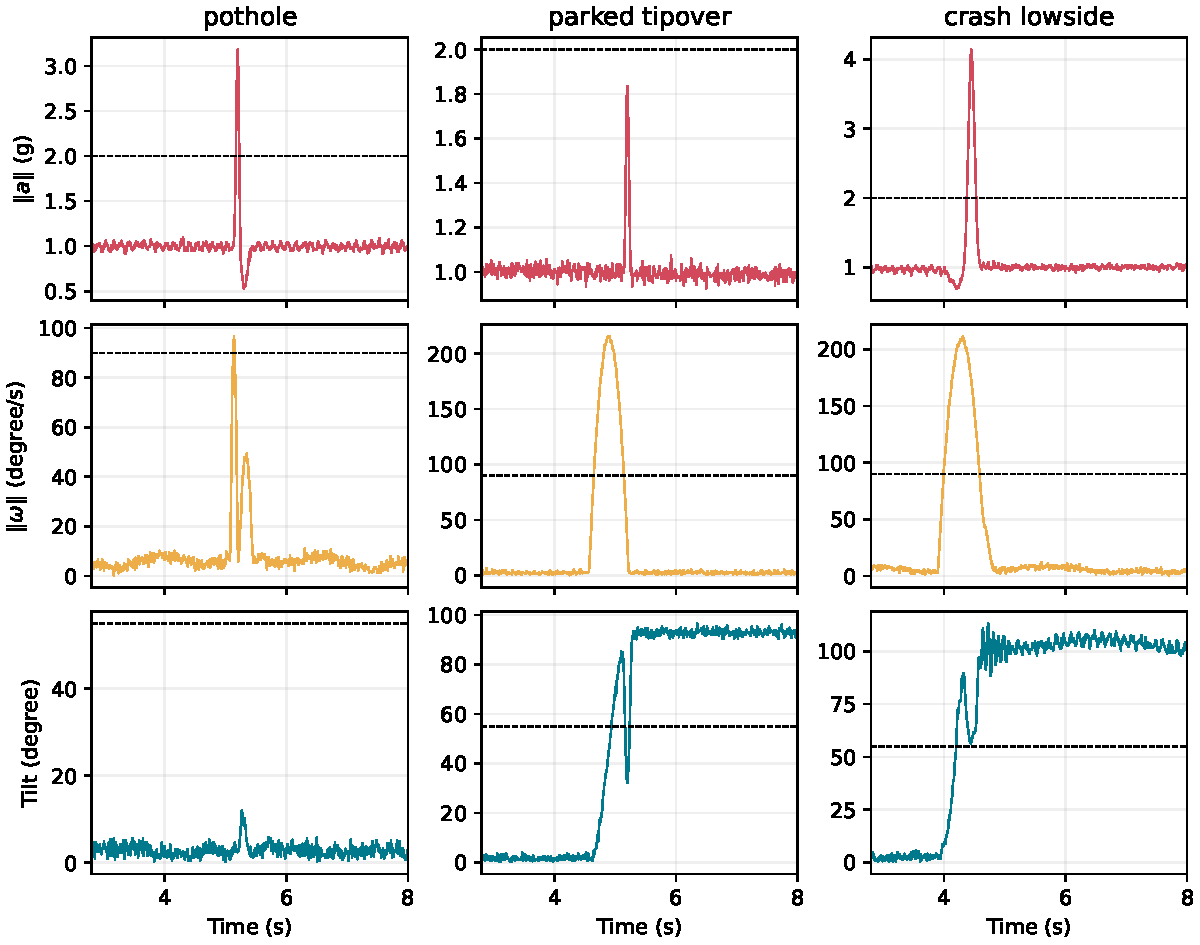
\includegraphics[width=0.93\textwidth]{../figures/simulated_profiles.pdf}
\caption{Representative pothole, parked tip-over, and low-side crash signals.
Dashed lines show the relevant CrashGuard gates.}
\label{fig:profiles}
\end{figure}

\subsection{Virtual-hardware output and cancellation}

On 4 September 2026, Wokwi CLI 0.26.1 executed the freshly compiled ESP32
binary once against the crash, pothole, and cancellation scenarios. All three
completed successfully. The crash run produced the following serial sequence;
the numeric candidate values are direct simulator output:

\begin{lstlisting}
READY sample_hz=100 battery=4.66V
RIDE_ACTIVE
CANDIDATE a=5.00 omega=240.6 tilt=2.3
ROTATION_CONFIRMED
CRASH_CONFIRMED countdown=15s
STATE COUNTDOWN
ALERT_DUE
BLYNK_EVENT_SKIPPED reason=not_configured
\end{lstlisting}

The pothole run produced \texttt{CANDIDATE\_REJECTED} and verified GPIO26 low.
For the cancellation case, the button is pressed after
\texttt{CRASH\_CONFIRMED}; the observed marker is
\texttt{ALERT\_CANCELLED}, GPIO26 returns low, remains low after a 16 s guard,
and no deadline marker is accepted. The test used no Blynk device credential,
so \texttt{BLYNK\_EVENT\_SKIPPED reason=not\_configured} is the expected and
observed offline handoff, not a cloud-delivery claim.

\section{Performance comparison}
\label{sec:performance}

For positive events, sensitivity is $TP/(TP+FN)$. For negative events,
specificity is $TN/(TN+FP)$ and false-positive rate is $FP/(TN+FP)$.
Accuracy is $(TP+TN)/N$. F1 is the harmonic mean of precision and sensitivity.
Wilson intervals are reported because even a zero observed false-positive
count does not establish a zero population rate~\cite{wilson1927interval}.

\begin{table}[H]
\centering
\small
\caption{Acceleration-only comparison versus CrashGuard on 675 generated events.}
\label{tab:performance}
\begin{tabular}{@{}lrrr@{}}
\toprule
Metric & Acceleration only & CrashGuard & Difference \\
\midrule
Accuracy & 54.8\% & 94.7\% & +39.9 points \\
Sensitivity / detection rate & 89.3\% & 76.0\% & -13.3 points \\
Specificity & 45.0\% & 100.0\% & +55.0 points \\
False-positive rate & 55.0\% & 0.0\% & -55.0 points \\
Precision & 31.7\% & 100.0\% & +68.3 points \\
F1 score & 0.468 & 0.864 & +0.396 \\
Median confirmation delay & 0 ms & 2310 ms & +2310 ms \\
\bottomrule
\end{tabular}
\end{table}

\begin{figure}[H]
\centering
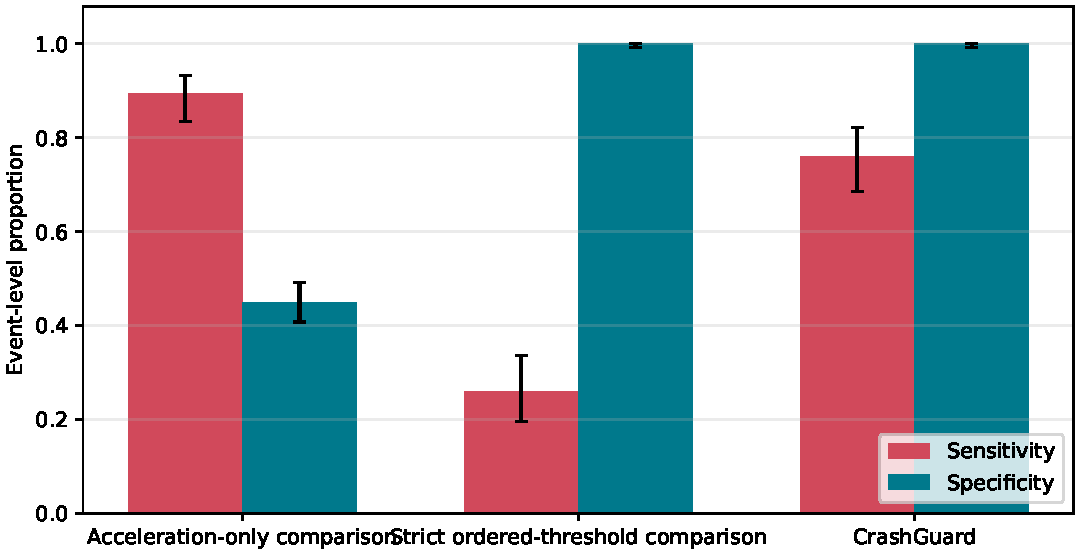
\includegraphics[width=0.78\textwidth]{../figures/performance_comparison.pdf}
\caption{Sensitivity and specificity with Wilson 95\% intervals. The third
bar group is a strict ordered-threshold comparison, not another CrashGuard
release. Intervals describe the simulated event counts only.}
\end{figure}

CrashGuard deliberately trades immediate response and some low-side
sensitivity for a large reduction in nuisance alerts. Its median 2.31 s
confirmation time is dominated by the required two-second final-rest hold.
The Blynk attempt occurs after the additional 15 s cancellation interval, so
the median candidate-to-cloud-attempt time is approximately 17.31 s before
network delay. This is appropriate for avoiding unwanted emergency alerts,
but it is too slow to claim pre-impact detection.

The observed confusion matrices are $(TP,TN,FP,FN)=(134,236,289,16)$ for the
acceleration-only method and $(114,525,0,36)$ for CrashGuard. CrashGuard's
sensitivity 95\% interval is [68.6\%, 82.1\%]. Its specificity lower Wilson
bound is 99.3\%, even though the observed value is 100\%. The result remains
synthetic and does not estimate false alerts per riding hour or kilometre.

\subsection{Comparison with the supplied base paper}

The supplied base paper reports a shin-mounted LSM6DSM at 50 Hz, 3.4 s
windows, a balanced CNN-transformer with focal loss, and human-fall test
sensitivity of 90.5\%, specificity of 94.5\%, and accuracy of 93.1\%
~\cite{tian2026transformer}. CrashGuard uses a handlebar MPU-6050 at 100 Hz and
a deterministic temporal state machine. Its 94.7\% simulated accuracy must
not be described as better than the paper's 93.1\%: sensing body, labels,
participants, events, splits, and evaluation units differ, and CrashGuard has
no physical test set. The transferable lesson is methodological: report
sensitivity and specificity separately, preserve temporal context, and match
the method to deployment constraints.

\section{IoT communication demonstration}
\label{sec:iot}

\begin{figure}[H]
\centering
\begin{tikzpicture}[
  node distance=5mm and 5mm,
  box/.style={draw,rounded corners,align=center,minimum width=27mm,
    minimum height=12mm,fill=blue!5,font=\small},
  arrow/.style={-Latex,thick}
]
\node[box] (sensor) {MPU-6050\\six-axis data};
\node[box,right=of sensor] (controller) {ESP32\\CrashGuard};
\node[box,right=of controller] (network) {Wi-Fi\\hotspot};
\node[box,right=of network] (cloud) {Blynk Cloud\\event};
\node[box,right=of cloud] (user) {Blynk app\\user alert};
\draw[arrow] (sensor) -- node[above,font=\scriptsize]{I\textsuperscript{2}C} (controller);
\draw[arrow] (controller) -- node[above,font=\scriptsize]{SSL} (network);
\draw[arrow] (network) -- node[above,font=\scriptsize]{Internet} (cloud);
\draw[arrow] (cloud) -- node[above,font=\scriptsize]{notification} (user);
\end{tikzpicture}
\caption{Required sensor-to-user chain. Solid arrows show the designed path;
only the sensor/controller and local-output segments have virtual-hardware
execution evidence in this project.}
\label{fig:iotchain}
\end{figure}

The firmware starts Wi-Fi asynchronously, preserves local detection when the
network is absent, and uses Blynk library 1.3.5 with the ESP32 SSL client. At
the alert deadline it requests a cloud connection and calls
\texttt{Blynk.logEvent("crash\_confirmed", description)}. Blynk requires the
same event code in the device template; the event settings control timeline
recording and user notifications~\cite{blynktemplate,blynkevents}. The code
prints \texttt{BLYNK\_EVENT\_SUBMITTED} only when the library reports an
authenticated connection. Since \texttt{logEvent} exposes no delivery
receipt, that marker is not treated as proof of cloud or phone receipt.

Wokwi provides the open \texttt{Wokwi-GUEST} network on channel 6 and Internet
access for an ESP32 simulation~\cite{wokwiwifi}. A dedicated test-device token
can exercise the same production code path. The current run deliberately used
no Blynk test-device credential: it validates the offline handoff without
sending a real event. No real credential appears in source or in this document.

\begin{table}[H]
\centering
\small
\caption{Communication-stage verification status.}
\begin{tabularx}{\textwidth}{@{}p{0.27\textwidth}p{0.19\textwidth}X@{}}
\toprule
Stage & Status & Evidence \\
\midrule
Sensor $\rightarrow$ controller & Verified virtually & MPU values drive the exact ESP32 detector path \\
Controller $\rightarrow$ alarm & Verified virtually & LED/piezo activation and button cancellation \\
Controller $\rightarrow$ Wi-Fi & Compile-verified & Credential-free and Blynk-enabled builds succeed \\
Wi-Fi $\rightarrow$ Blynk & Not measured & Opt-in scenario exists; no current authenticated run \\
Blynk $\rightarrow$ user & Not measured & Requires configured event, notification settings, and a real recipient \\
\bottomrule
\end{tabularx}
\end{table}

\section{Dashboard and user interface}
\label{sec:dashboard}

Figure~\ref{fig:dashboard} is a reproducible dashboard rendered from the
low-side exemplar in the deterministic dataset. It displays acceleration,
angular rate, tilt, detector status, local alarm state, countdown, and cloud
test status. It is a replay UI, not a screenshot of Blynk Cloud.

\begin{figure}[H]
\centering
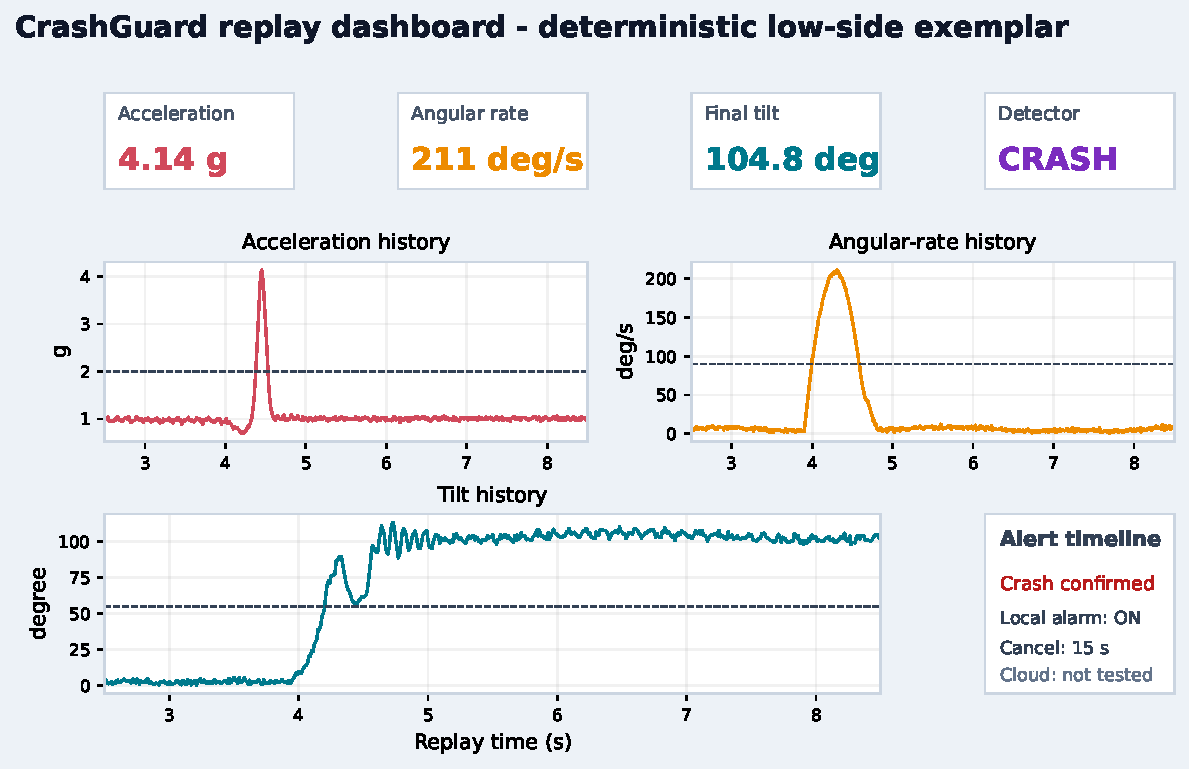
\includegraphics[width=\textwidth]{figures/replay_dashboard.pdf}
\caption{Replay dashboard generated directly from deterministic six-axis data.}
\label{fig:dashboard}
\end{figure}

For a Blynk dashboard, datastreams should use virtual pins rather than physical
GPIO identifiers. Blynk defines datastreams as time-stamped channels and binds
dashboard widgets to them~\cite{blynktemplate,blynkdata}. Telemetry should be
published on a controlled timer rather than every 100 Hz detector iteration,
which would spam the service. Table~\ref{tab:blynkmap} defines the intended
one-hertz dashboard mapping.

\begin{table}[H]
\centering
\small
\caption{Blynk template and dashboard mapping.}
\label{tab:blynkmap}
\begin{tabularx}{\textwidth}{@{}p{0.08\textwidth}p{0.23\textwidth}p{0.16\textwidth}p{0.20\textwidth}X@{}}
\toprule
Pin & Datastream & Type/range & Widget & Update policy \\
\midrule
V0 & Acceleration magnitude & Double, 0--16 g & Gauge + chart & 1 Hz \\
V1 & Angular-rate magnitude & Double, 0--2000 $\degree$/s & Gauge + chart & 1 Hz \\
V2 & Tilt & Double, 0--180 $\degree$ & Gauge + chart & 1 Hz \\
V3 & Detector-state code & Integer, 0--4 & Label / status & On change \\
V4 & Battery voltage & Double, 0--5 V & Gauge & Every 60 s \\
Event & \texttt{crash\_confirmed} & Critical event & Timeline + notification & Once per uncancelled incident \\
\bottomrule
\end{tabularx}
\end{table}

The released firmware currently implements the event path, not continuous V0
through V4 publication. Therefore, the Blynk telemetry dashboard is a precise
configuration and next implementation step, while the replay dashboard is the
only dashboard with actual values in this report.

\section{Fault handling}
\label{sec:faults}

\subsection{Fault 1: sensor unavailable or read failure}

At startup, the ESP32 probes I\textsuperscript{2}C address \texttt{0x68}. A
failed probe prints \texttt{FATAL\_MPU6050\_\allowbreak NOT\_FOUND} and enters a safe stop,
so uninitialized data cannot generate a crash event. During operation, a
14-byte burst-read failure prints \texttt{WARN\_MPU6050\_\allowbreak READ\_FAILED}, returns
from the loop iteration, and does not update the state machine. Stationary
calibration also rejects gravity outside 0.85--1.15 g or gyro RMS above
5 $\degree$/s and retries instead of accepting a bad reference.

This is fail-silent detection: it prevents fabricated events but temporarily
loses coverage. The source path and target compilation are verified; physical
wire removal and current-source Wokwi disconnect injection were not executed.
The correct enhancement is a latched sensor-health state, retry counter,
visible fault LED pattern, and controlled bus reinitialization.

\subsection{Fault 2: Wi-Fi or Blynk unavailable}

Network failure cannot block the initial crash decision, local alarm, or cancel
button. At the deadline, the firmware distinguishes four outcomes: event
submitted, Blynk not configured, Wi-Fi unavailable, and cloud unavailable.
Unavailable outcomes produce an explicit serial marker and never claim that a
notification was sent. The local alarm remains active until acknowledged.

The credential-free build is current compile evidence, and the fresh Wokwi
run demonstrated local alarm behavior without cloud credentials. A real
Wi-Fi-drop/Blynk-recovery run remains outstanding. The main functional gap is
that the current event attempt is one-shot; a production design should queue
the incident in nonvolatile storage and retry with capped exponential backoff.

\begin{table}[H]
\centering
\small
\caption{Fault detection, safe response, and residual risk.}
\begin{tabularx}{\textwidth}{@{}p{0.19\textwidth}p{0.24\textwidth}p{0.25\textwidth}X@{}}
\toprule
Fault & Detection & Current response & Residual risk \\
\midrule
MPU absent at boot & I\textsuperscript{2}C probe fails & Fatal marker; safe stop & No automatic field recovery \\
MPU read failure & Burst length/status invalid & Warning; skip detector update & Detection gap; repeated logs \\
Bad calibration motion & Gravity/gyro bounds fail & Retry calibration & Device remains unavailable until still \\
Wi-Fi unavailable & ESP32 link state not connected & Explicit skipped marker; local alarm continues & Incident not queued for retry \\
Blynk unavailable & Authenticated connect times out & Explicit cloud-unavailable marker & User receives no remote alert \\
\bottomrule
\end{tabularx}
\end{table}

Power and actuator faults are not yet detected. The ADC voltage is printed at
startup but no calibrated low-battery cutoff exists, and the ESP32 cannot
confirm that a piezo actually produced sound without current or acoustic
feedback. These are documented gaps rather than passed tests.

\section{Expected versus actual results and deviations}
\label{sec:deviations}

\begin{table}[H]
\centering
\footnotesize
\caption{Expectation, observed result, and interpretation.}
\begin{tabularx}{\textwidth}{@{}p{0.25\textwidth}p{0.25\textwidth}p{0.20\textwidth}X@{}}
\toprule
Expectation & Actual result & Deviation & Explanation / decision \\
\midrule
Reject ordinary and abnormal non-crashes & 0/525 CrashGuard false positives & Meets finite simulation set & Temporal correlation, ride qualification, and final rest reject isolated motion \\
Detect high-energy crashes & 75/75 high-side detected & Meets generated set & Strong impact/rotation/rest pattern crosses all gates \\
Detect lower-energy crashes & 39/75 low-side detected & 36 false negatives & Fixed gates and timing miss weaker profiles; do not retune on the same generator \\
Alert immediately after confirmation & Local alarm immediate; cloud attempt after 15 s & Intentional 15 s delay & Cancellation reduces unwanted remote alerts \\
Deliver Blynk alert to user & Event path compile-verified; receipt not measured & Incomplete end-to-end evidence & Requires test device, network, configured event, and phone \\
Operate for about 13 h & Only a power-budget estimate exists & Runtime unmeasured & Converter efficiency and real duty cycle need hardware logging \\
Recover from sensor/network faults & Safe skip/stop exists; automatic retry limited & Partial & Add health state, persistence, retry, and diagnostics \\
\bottomrule
\end{tabularx}
\end{table}

The largest favorable deviation relative to the acceleration-only method is
false-positive control: 289 simulated false alarms are removed. The cost is 20
additional false negatives (36 instead of 16) and a 2.31 s median confirmation
delay. In a safety system this is not automatically a good trade; it defines a
candidate operating point that must be evaluated on target-domain physical
data before selection.

\section{Resource, energy, and network evaluation}

The credential-free ESP32 build uses 392,955 bytes of flash (29\%) and 29,808
bytes of static RAM (9\%). The Blynk SSL build uses 1,040,295 bytes (79\%) and
49,124 bytes (14\%). Both fit the selected target, but the SSL certificate and
network stack leave much less flash margin. These figures do not include
worst-case stack/heap fragmentation or long-duration behavior.

At an estimated average 5 V load of 120 mA, the load power is 0.60 W. Assuming
a 3.7 V, 2600 mAh cell, 90\% usable capacity, and 90\% boost efficiency gives

\begin{equation}
 I_{cell}\approx\frac{5(0.120)}{3.7(0.90)}=0.180\ \mathrm{A},\qquad
 t\approx\frac{2.6(0.90)}{0.180}=13.0\ \mathrm{h}.
\end{equation}

This is a sizing estimate, not measured energy consumption. Network latency is
also not reported: compiler success and a simulated alert deadline provide no
round-trip timing to Blynk. Physical evaluation should record detection time,
Wi-Fi association, TLS connection, Blynk timeline arrival, and phone
notification arrival using synchronized clocks.

\section{Future enhancements}
\label{sec:future}

The following work is prioritized by safety evidence rather than novelty:

\begin{enumerate}
  \item \textbf{Physical target-domain dataset.} Instrument a rigid handlebar
        mount; bench-check scale and orientation; collect ordinary riding over
        braking, turns, potholes, speed breakers, weather, payload, and mount
        variations; then collect unmanned soft-containment tip/drop trials.
        Freeze thresholds before a held-out route and report false alerts per
        hour and kilometre.
  \item \textbf{Reliable event delivery.} Store an uncancelled incident in
        nonvolatile memory, attach monotonic time and delivery state, retry with
        capped backoff, clear only after a verifiable server acknowledgement,
        and prevent event storms. Blynk documents a per-device event limit, so
        one event per incident and rate control are required~\cite{blynkevents}.
  \item \textbf{Complete dashboard telemetry.} Publish V0--V4 at controlled
        rates, enable history where appropriate, add connection-age and sensor-
        health indicators, and validate web/mobile widgets with a dedicated
        test device.
  \item \textbf{Fault diagnostics.} Add a sensor retry state, watchdog,
        low-battery threshold with hysteresis, brownout log, alarm-current
        feedback, and visible degraded-mode indication.
  \item \textbf{Location integration.} Add GNSS or a companion-phone protocol.
        A hotspot alone does not expose phone GPS; coordinates must never be
        fabricated.
  \item \textbf{Model improvement after data collection.} Compare the frozen
        state machine with small trees or quantized temporal models using
        subject/route/vehicle-separated evaluation. The supplied transformer's
        50 Hz human-shin result is architectural guidance, not training data
        for this motorcycle problem.
  \item \textbf{Security and maintenance.} Keep device tokens outside source,
        use TLS, rotate compromised tokens, restrict Blynk device privileges,
        record firmware identity, and define a signed update and rollback plan.
\end{enumerate}

\section{Limitations, safety, and conclusion}

The generated signals omit frame flexibility, mount slip, engine harmonics,
temperature drift, varied impact points, rider separation, traffic, and radio
conditions. The public archive contains only four controlled falls. The
generator and thresholds were co-developed, Wokwi does not simulate vehicle
mechanics or the power circuit, the Blynk user path lacks an authenticated
current run, and no energy or latency measurement exists. The prototype is
not a certified automotive, medical, or emergency device. Deliberate
public-road crash tests would be unsafe.

Within these limits, CrashGuard demonstrates an integrated and repeatable
sensor-to-local-alarm system with rider cancellation and a compile-verified
Blynk event path. It passes seven of ten listed cases completely and exposes
the remaining gaps: low-side sensitivity, end-to-end cloud proof, and physical
fault injection. Compared with acceleration alone, it improves simulated
accuracy from 54.8\% to 94.7\% and removes 289 false positives, while reducing
sensitivity and adding confirmation delay. The next defensible milestone is
not a stronger accuracy claim; it is a physical holdout study plus an
authenticated, timestamped Blynk delivery test.

\clearpage
{\small
\bibliography{references}
}

\end{document}
